У даному розділі досліджено плоска динамічна задача теорії пружності для прямокутної області,
за другої основної задачі теорії пружності на бічних гранях.

Вихідна задача зведена до одновимірної задачі у просторі трансформант за допомогою інтегрального перетворення Фур'є.
Отримана крайова задача розв'язана точно за допомогою методу матрично диференціального числення,
фундаментальний розв'язок представлений як інтеграл по замкненому контору, який в свою чергу, був знайденний за допомогою теоремі про лишки.
Побудована матриця-функція Гріна як комбінація фундаментальних базисних розв'язків задачі у просторі трансформант.
Остаточний вигляд для функцій переміщеннь та напружень отриман шляхом оберненого перетворення Фур'є.
Побудовано та розв'язано сінгульрне інтегральне рівняння відносно невідомої функції шляхом викорстання методу ортагональних многочленів, та зведення рівнняння до бескінечної алгебричної системи,
яка в подальшому була розв'язана методом редукціі \cite{popov_3}.

Проведено чисельний аналіз отриманих функцій переміщень та напружень для різних розмірів прямокутної області та різних видів навантаження.

\subsection{Постановка задачі}
\begin{figure}[h]
    \begin{center}
        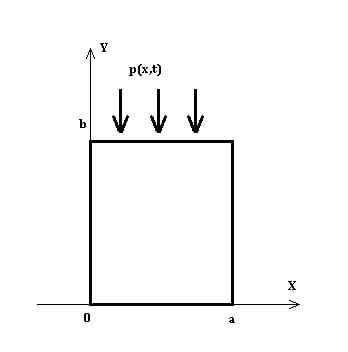
\includegraphics[scale=1]{images/geometry/image_2.jpg}
    \end{center}
    \caption{Геометрія проблеми}\label{geom_dynamic_2}
\end{figure}
Розглядається пружна сама прямокутна область (Рис: \ref{geom_dynamic_1}), яка займає облась,
що описується у декартовій системі координат співвідношенням $0 \le x \le a$, $0 \le y \le b$.

До прямокутної області на грані $y=b$ додане нормальне навантаження
\begin{equation}
    \sigma_y(x, y, t) |_{y=b} = -p(x, t), \quad  \tau_{xy}(x,y,t) |_{y=b} =0
\end{equation}
де $p(x,t)$ відома функція.
На бічних гранях виконується умова другої основної задачі теорії пружності
\begin{equation}
    u(x,y,t) |_{x=\pm a} = 0, \quad v(x,y,t) |_{x=\pm a} =0
\end{equation}
На нижній грані виконуються наступні умови
\begin{equation}
    v(x,y,t) |_{y=0} = 0, \quad \tau_{xy}(x,y,t) |_{y=0} =0
\end{equation}
Розглядаються наступні рівняння рівноваги Ламе:
\begin{equation}
    \begin{cases}
        \frac{\partial^2 u(x,y,t)}{\partial x^2} + \frac{\partial^2 u(x,y,t)}{\partial y^2} + \mu_0 (\frac{\partial^2 u(x,y,t)}{\partial x^2} + \frac{\partial^2 v(x,y,t)}{\partial x\partial y}) = \frac{1}{c_1^2} \frac{\partial^2 u(x,y,t)}{\partial t^2} \\
        \frac{\partial^2 v(x,y,t)}{\partial x^2} + \frac{\partial^2 v(x,y,t)}{\partial y^2} + \mu_0 (\frac{\partial^2 u(x,y,t)}{\partial x \partial y} + \frac{\partial^2 v(x,y,t)}{\partial y^2}) = \frac{1}{c_2^2} \frac{\partial^2 v(x,y,t)}{\partial t^2} \\
    \end{cases}
\end{equation}

Будемо розглядати випадок гармонічних коливань, тому можемо предствавити функції у наступному вигляді:
\begin{equation}
    u(x,y,t) = u(x,y) e^{i \omega t}, \quad v(x,y,t) = v(x,y) e^{i \omega t}, \quad p(x,t) = p(x) e^{i \omega t}
\end{equation}
Таким чином отримаємо наступні рівняння рівноваги:
\begin{equation}\label{lame_dynamic_2}
    \begin{cases}
        \frac{\partial^2 u(x,y)}{\partial x^2} + \frac{\partial^2 u(x,y)}{\partial y^2} + \mu_0 (\frac{\partial^2 u(x,y)}{\partial x^2} + \frac{\partial^2 v(x,y)}{\partial x\partial y}) = -\frac{\omega^2}{c_1^2}  u(x,y) \\
        \frac{\partial^2 v(x,y)}{\partial x^2} + \frac{\partial^2 v(x,y)}{\partial y^2} + \mu_0 (\frac{\partial^2 u(x,y)}{\partial x \partial y} + \frac{\partial^2 v(x,y)}{\partial y^2}) = -\frac{\omega^2}{c_2^2} v(x,y) \\
    \end{cases}
\end{equation}
Також, щоб розв'язати поставлену задачу буде розглянута тільки половона прямокутної області $0 \le x \le a$, $0 \le y \le b$
та використовуючи властивості симметрії граничні умови в результаті будуть мати вигляд:
\begin{equation}\label{bound_dynamic_2}
    \begin{cases}
        \sigma_y(x, y) |_{y=b} = -p(x, t), \quad  \tau_{xy}(x,y) |_{y=b} =0 \\
        v(x,y) |_{y=0} = 0, \quad \tau_{xy}(x,y) |_{y=0} = 0 \\
        u(x,y) |_{x=0} = 0, \quad \tau_{xy}(x,y) |_{x=0} = 0 \\
        u(x,y) |_{x=a} = 0, \quad v(x,y) |_{x=a} = 0
    \end{cases}
\end{equation}

\subsection{Зведеня задачі до одновимірної у просторі трансформант}
Для того, щоб звести задачу до одновимірної задачі, використаєм інтегральне перетворення Фур'є по змінній $x$ у до рівнянь (\ref{lame_dynamic_2}) наступному вигляді:
\begin{equation}
    \begin{pmatrix}
        u_n(y) \\
        v_n(y)
    \end{pmatrix} = \int_{0}^{a} 
    \begin{pmatrix}
        u(x,y) sin(\alpha_n x) \\
        v(x,y) cos(\alpha_n x)
    \end{pmatrix} dx, \quad \alpha_n = \frac{\pi n}{a}
\end{equation}

Для цього помножим перше та друге рівняння (\ref{lame_dynamic_2}) на $sin(\alpha_n x)$ та $cos(\alpha_n x)$ відповідно та проінтегруєм по змінній $x$ на інтервалі $0 \le x \le a$.
Покрокове інтегрування рівняння (\ref{lame_dynamic_2}) наведено у (\nameref{ap_A}).
Отримана система рівнянь задачі у просторі трансформант:
\begin{equation}\label{transf_dynamic_2}
    \begin{cases}
        u_n^{''}(y) - \alpha_n \mu_0 v_n^{'}(y) + (-\alpha_n^2 -\alpha_n^2 \mu_0 + \frac{\omega^2}{c_1^2}) u_n(y) = 0 \\
        (1 + \mu_0) v_n^{''}(y) + \alpha_n \mu_0 u_n^{'}(y) + (- \alpha_n^2 + \frac{\omega^2}{c_2^2}) v_n(y) = -cos(\alpha_n) f(y)\\
    \end{cases}
\end{equation}
Де $f(y) = \frac{\partial v(x,y)}{\partial x}|_{x=a}$ - невідома функція

Застосовуючи інтегральне перетворення до граничних умов,
отримаємо наступні умови задачі у просторі трансформант
\begin{equation}\label{transf_bound_dynamic_2}
    \begin{cases}
        \left( (2G + \lambda)v_n^{'}(y) + \alpha_n \lambda u_n(y) \right)|_{y=b} = -p_n \\
        \left(u_n^{'}(y) - \alpha_n v_n(y)  \right)|_{y=b} = 0 \\
        v_n(y)|_{y=0} = 0 \\
        \left(u_n^{'}(y) - \alpha_n v_n(y)  \right)|_{y=0} = 0
    \end{cases}
\end{equation}
Де $p_n = \int_{0}^{a} p(x) cos(\alpha_n x) dx$

\subsection{Зведення задачі у просторі трансформант до матрично-векторної форми}
Для того щоб розв'язати задачу у простосторі трансформант, перепишмо її у матрично-векторній формі.
Рівняння рівноваги (\ref{transf_dynamic_2}) запишемо у наступному вигляді:
\begin{align}\label{transf_mat_dynamic_2}
    &L_2\left[ Z_n(y) \right] = A * Z_n^{''}(y) + B * Z_n^{'}(y) + C * Z_n(y) \nonumber \\
    &L_2\left[ Z_n(y) \right] = F_n(y)
\end{align}
Де
\begin{equation*}
    A = \begin{pmatrix}
        1 & 0 \\
        0 & 1 + \mu_0
    \end{pmatrix}, \quad
    B = \begin{pmatrix}
        0 & -\alpha_n \mu_0 \\
        \alpha_n \mu_0 & 0
    \end{pmatrix},
\end{equation*}
\begin{equation*}
    \centering
    C = \begin{pmatrix}
        -\alpha_n^2 -\alpha_n^2 \mu_0 + \frac{\omega^2}{c_1^2} & 0 \\
        0 & -\alpha_n^2 + \frac{\omega^2}{c_2^2}
    \end{pmatrix},
\end{equation*}
\begin{equation*}
    Z_n(y) = \begin{pmatrix}
        u_n(y) \\
        v_n(y)
    \end{pmatrix}, \quad 
    F_n(y) = \begin{pmatrix}
        0 \\
        - cos(\alpha_n a) f(y)
    \end{pmatrix}
\end{equation*}
Граничні умови (\ref{transf_bound_dynamic_2}) запишемо у наступному вигляді:
\begin{align}\label{transf_bound_mat_dynamic_2}
    &U_i\left[ Z_n(y) \right] = E_i * Z_n^{'}(b_i) + F_i * Z_n(b_i) \nonumber \\
    & U_i\left[ Z_n(y) \right] = D_i
\end{align}
Де $i = \overline{0, 1}$, $b_0 = b$, $b_1 = 0$,
\begin{equation*}
    E_0 = \begin{pmatrix}
        1 & 0 \\
        0 & 2G + \lambda
    \end{pmatrix}, \quad
    F_0 = \begin{pmatrix}
        0 & -\alpha_n \\
        \alpha_n \lambda & 0
    \end{pmatrix}, \quad
\end{equation*}
\begin{equation*}
    E_1 = \begin{pmatrix}
        1 & 0 \\
        0 & 0
    \end{pmatrix}, \quad
    F_1 = \begin{pmatrix}
        0 & -\alpha_n \\
        0 & 1
    \end{pmatrix}, \quad
\end{equation*}
\begin{equation*}
    D_0 = \begin{pmatrix}
        0 \\
        -p_n
    \end{pmatrix}, \quad
    D_1 = \begin{pmatrix}
        0 \\
        0
    \end{pmatrix}, \quad
\end{equation*}